%Math template by Kaushik Srinivasan

\documentclass[11pt]{article}




%----------%
%  Basics  %
%----------%


%  Specfies basic information.
%  In the metadata section of the preamble, you can specify the subject and a list of keywords for the PDF.
%
\newcommand{\coursetitle}{AMS 553.430 - Introduction to Statistics}
\newcommand{\lecturer}{Dwijavanti P Athreya}
\newcommand{\notetaker}{Kaushik Srinivasan}
\newcommand{\notetakersemail}{ksriniv4@jhu.edu}
\newcommand{\courseterm}{Fall 2018}
\newcommand{\institution}{Johns Hopkins University}


%  array provides more column styles for the tabular and array environments.
%  (http://ctan.org/pkg/array)
%
%  parskip sets block paragraphs as the default, instead of indentation.
%  (http://www.ctan.org/pkg/parskip)
%
\usepackage[margin=1in]{geometry}
\usepackage{amsmath,amssymb,amsthm,amsfonts,array,parskip}


%  Allows equation, align, gather, etc. environments to split across pages.
\allowdisplaybreaks


%  Sets date formatting to the ISO 8601 standard, YYYY-MM-DD.
\usepackage{datetime} \renewcommand{\dateseparator}{-} \yyyymmdddate


%---------%
%  Fonts  %
%---------%


%  Defines \cal for standard calligraphy, \eucal for Euler calligraphy, and \frak for Fraktur.
\usepackage{eucal}  \let\eucal\mathcal  \let\cal\CMcal  \renewcommand{\frak}{\mathfrak}


%  Removes ligatures (e.g. the connection ordinarily made between the two f's in "differentiable").
%\usepackage{microtype} \DisableLigatures{encoding=*,family=*}


%  Removes extra space after periods.




%-------------------------------%
%  Environments and Sectioning  %
%-------------------------------%


%  Defines some standard theorem environments, in both numbered and non-numbered versions. The numbering of each enviroment will be reset for each lecture.
\newcounter{lecture}       \setcounter{lecture}{-1}
\newcounter{tN}[lecture]   \newcounter{dN}[lecture]
\newcounter{lN}[lecture]   \newcounter{rN}[lecture]
\newcounter{cN}[lecture]   \newcounter{eN}[lecture]
\newcounter{pN}[lecture]

\newtheorem*{theorem}{Theorem}          \newtheorem{theorem-N}[tN]{Theorem}
\newtheorem*{lemma}{Lemma}              \newtheorem{lemma-N}[lN]{Lemma}
\newtheorem*{corollary}{Corollary}      \newtheorem{corollary-N}[cN]{Corollary}
\newtheorem*{proposition}{Proposition}  \newtheorem{proposition-N}[pN]{Proposition}

\theoremstyle{definition}
\newtheorem*{definition}{Definition}    \newtheorem{definition-N}[dN]{Definition}
\newtheorem*{remark}{Remark}            \newtheorem{remark-N}[rN]{Remark}
\newtheorem*{example}{Example}          \newtheorem{example-N}[eN]{Example}
\newtheorem*{claim}{Claim}          \newtheorem{claim-N}[cN]{Claim}

% Modifies the spacing above theorem environments, which is messed up during the parskip package

\makeatletter \def\thm@space@setup{\thm@preskip=\parskip \thm@postskip=0pt} \makeatother

%Modifies the spacing above the proof environment

\makeatletter \renewenvironment{proof}[1][\proofname]{\pushQED{\qed}\normalfont
\partopsep=\z@skip \topsep=\z@skip \trivlist \item[\hskip\labelsep\itshape #1\@addpunct{.}]
\ignorespaces}{\popQED\endtrivlist\@endpefalse} \makeatother

\renewcommand{\qedsymbol}{\rule{0.7em}{0.7em}}

%Removes extra space before and after section headings

\usepackage[compact]{titlesec}

%% PICTURES AND DIAGRAMS


\usepackage[usenames, dvipsnames]{xcolor}
\definecolor{myred}{rgb}{0.9,0.2,0.2}
\definecolor{mygreen}{rgb}{0.2,0.6,0.2}
\definecolor{myblue}{rgb}{0.2,0.2,0.8}
\usepackage{caption}

%graphicx provides advanced graphics options

\usepackage{graphicx}
\graphicspath{ {./images/} }

% tikz is for drawing all sorts of pictures and diagrams

\usepackage{tikz}
\usepackage{tabularx}
\usetikzlibrary{decorations.text}
\newcommand{\tikzmark}[2]{%
    \tikz[remember picture,baseline=-2pt]
    \node[circle,red,draw,text=black,anchor=center,inner sep=1pt] (#1) {$#2$};}
\usepackage{tikz-cd}
\usepackage{pgf, pgfplots}
\usetikzlibrary{arrows,calc,decorations,decorations.markings,fadings,positioning,patterns,shapes}
\tikzset{>=latex}
\tikzstyle{mypoint}=[inner sep=0pt,outer sep=0pt,minimum size=5pt,fill,circle]
% for circled commands
\usepackage{enumitem}
%\begin{enumerate[label=\protect\circled{\arabic*}]
\newcommand*\circled[1]{\tikz[baseline=(char.base)]{\node[shape=circle,draw,inner sep=2pt] (char) {#1};}}

% HORIZONTAL LINES

\newcommand{\redhline}{\vspace{-0.1in}{\color{myred}{\rule{\textwidth}{0.02in}}}}


%------------------------%
%  Commands and Symbols  %
%------------------------%


%  Creates commands by running over a comma-separated list. For example,
%
%     \forcsvlist{\define{\newcommand}{\textbf}{bold}}{A,B}
%
%  would create
%
%     \newcommand{\boldA}{\textbf{A}}    \newcommand{\boldB}{\textbf{B}}
%
%  (http://tex.stackexchange.com/a/5776/20882)
%
\usepackage{etoolbox}
\newcommand{\define}[4]{\expandafter#1\csname#3#4\endcsname{#2{#4}}}
\forcsvlist{\define{\DeclareMathOperator}{}{}}{im,coker,rad,nil,Ann,Ass,codim,Spec,mSpec,diam,ord,Supp,supp,disc,Ob,vol,rank,Sym,Alt,Ind}
\forcsvlist{\define{\newcommand}{\mathrm}{}}{Hom,Mor,id,GL,SL,SO,SU,U,M,Mat,Ext,Tor,Res,Cor,Inf,End,Irr,Aut,Gal,lcm,tr,sign,triv,diag,Map,op,ev,act,alg,sep,unr,nr,ab}

%  Creates commands for some names of categories in the sans-serif font.
\forcsvlist{\define{\newcommand}{\mathsf}{}}{Set,Grp,Ab,CRing,Mod,Vect,Cat,Top,PreSh,Sh,Sch,Nat,Fun,Diff}

%  Creates commands for some blackboard bold letters.
\forcsvlist{\define{\newcommand}{\mathbb}{}}{N,Z,Q,R,C,F,G,T,A,B,D}


%  Saves the section symbol, paragraph symbol, Hungarian accent, and Scandanavian O in the macros \SS, \PP, \HH, and \OO, then redefines \S, \P, \H, and \O to be the corresponding blackboard bold letters.
%
\let\SS\S  \let\PP\P  \let\HH\H  \let\OO\O
\forcsvlist{\define{\renewcommand}{\mathbb}{}}{S,P,H,O}


%  latexsym defines some alternative versions of amssymb symbols.
%  (http://www.bakoma-tex.com/doc/latex/base/latexsym.pdf)
%
\usepackage{latexsym}

\usepackage{accents}
\newcommand{\Ylines}{\underaccent{\bar}{\bar{Y}}}
\newcommand{\Xlines}{\underaccent{\bar}{\bar{X}}}
\newcommand{\Lim}[1]{\raisebox{0.5ex}{\scalebox{0.8}{$\displaystyle \lim_{#1}\;$}}}
%  Defines a copyright symbol that is a bit nicer than the built-in one.
\newcommand{\mycopyrightsymbol}{\raisebox{-0.3ex}{\tikz{\node[inner sep=0pt,outer sep=0pt] at (0,0) {\textsc{c}};\draw (0,0) circle (0.18);}}}


%  Defines commands for real and complex projective space.
\newcommand{\RP}{\mathbb{R}\mathrm{P}}  \newcommand{\CP}{\mathbb{C}\mathrm{P}}


%  Defines a bordered matrix with square bracket delimiters instead of parentheses.
%  (http://tex.stackexchange.com/questions/55054)
%
\let\bbordermatrix\bordermatrix
\patchcmd{\bbordermatrix}{8.75}{4.75}{}{}
\patchcmd{\bbordermatrix}{\left(}{\left[}{}{}
\patchcmd{\bbordermatrix}{\right)}{\right]}{}{}

%% MATH STUFF

\usepackage{relsize}
\usepackage{cancel}

%Box Colour (https://tex.stackexchange.com/questions/122945/coloured-shadowed-boxes-around-equations)
\usepackage[skins,theorems]{tcolorbox}
\tcbset{highlight math style={enhanced, colframe=red,colback=white,arc=0pt,boxrule=1pt}}
  


% Math Symbol Aliases

\newcommand{\bs}{\backslash}
\newcommand{\subeq}{\subseteq}
\newcommand{\supeq}{\supseteq}
\newcommand{\subneq}{\subsetneq}
\newcommand{\supneq}{\supsetneq}
\newcommand{\derivativex}{\dfrac{\partial}{\partial x}}
\newcommand{\customderiv}[2]{\dfrac{\partial #1}{\partial #2}}


% Accents

\newcommand{\openset}{\,\open{\subeq}\,}
\newcommand{\open}[1]{\mathring{#1}}
\newcommand{\clos}[1]{\overline{#1}}
\newcommand{\resid}[1]{\overline{#1}}
\newcommand{\cover}[1]{\widetilde{#1}}
\newcommand{\overbar}[1]{%
  \mkern 1.5mu\overline{\mkern-1.5mu#1\mkern-1.5mu}\mkern 1.5mu%
}

%  Defines a bordered matrix with square bracket delimiters instead of parentheses.
%  (http://tex.stackexchange.com/questions/55054)
%
\let\bbordermatrix\bordermatrix
\patchcmd{\bbordermatrix}{8.75}{4.75}{}{}
\patchcmd{\bbordermatrix}{\left(}{\left[}{}{}
\patchcmd{\bbordermatrix}{\right)}{\right]}{}{}

%  Calls one of the mathabx font families so that it is possible to use its symbols without making a global change.
%  (http://www.ctan.org/pkg/mathabx)
%  (http://tex.stackexchange.com/questions/14386)
%
\DeclareFontFamily{U}{mathb}{\hyphenchar\font45}
\DeclareFontShape{U}{mathb}{m}{n}{<5> <6> <7> <8> <9> <10> gen * mathb
<10.95> mathb10 <12> <14.4> <17.28> <20.74> <24.88> mathb12}{}
\DeclareSymbolFont{mathb}{U}{mathb}{m}{n}

% Defines circular arrows

\DeclareFontFamily{U}{mathb}{\hyphenchar\font45}
\DeclareFontShape{U}{mathb}{m}{n}{<5> <6> <7> <8> <9> <10> gen * mathb
<10.95> mathb10 <12> <14.4> <17.28> <20.74> <24.88> mathb12}{}
\DeclareSymbolFont{mathb}{U}{mathb}{m}{n}

%  Defines circular arrows.
\DeclareMathSymbol{\lcirclearrow}{0}{mathb}{'366}
\DeclareMathSymbol{\rcirclearrow}{0}{mathb}{'367}
\newcommand{\leftcirclearrow}{\mathrel{\ensuremath{\raisebox{0.1ex}{\scalebox{0.9}{\rotatebox[origin=c]{90}{$\lcirclearrow$}}}}}}
\newcommand{\rightcirclearrow}{\mathrel{\ensuremath{\raisebox{0.1ex}{\scalebox{0.9}{\rotatebox[origin=c]{270}{$\rcirclearrow$}}}}}}

% Semantic names for some common math Symbols.

%-----------------------------------%
%  Things Specific to Course Notes  %
%-----------------------------------%


%  Formatting for the table of contents. The first line allows for multi-column environments, the second line removes the heading "Contents".
\usepackage{multicol} \setlength{\columnsep}{3cm}
\makeatletter \renewcommand\tableofcontents{\@starttoc{toc}} \makeatother


%  Sets the page style.
\usepackage{fancyhdr}
\pagestyle{fancy}
\renewcommand{\headrulewidth}{0pt}
\renewcommand{\footrulewidth}{0.5pt}
\setlength{\headheight}{14pt}
\lfoot{\parbox[t]{1in}{\centering Last edited\\ \today}}
\cfoot{\parbox[t]{3in}{\centering \coursetitle}}
\rfoot{\parbox[t]{0.9in}{\centering Page \thepage\\ Lecture \arabic{lecture}}}


%  Sets the inputs for \maketitle.
\author{Lectures by \lecturer\\ Notes by \notetaker}
\title{\coursetitle}
\date{\institution\\ \courseterm}


%  Defines headings for each day's notes.
\newcommand{\classheader}[1]{\stepcounter{lecture}\newpage\section*{Lecture \arabic{lecture} (#1)}
\phantomsection \addcontentsline{toc}{section}{Lecture \arabic{lecture} (#1)}}
	
% Misc additions to Template

% http://tex.stackexchange.com/questions/18359
\pgfplotsset{compat=newest}

\newcommand{\Cinfty}{\ensuremath{C^{\infty}}}
\newcommand{\Crit}{\mathrm{Crit}}
\usepackage{mathtools}
\newcommand{\Or}{\mathrm{Or}}
\renewcommand{\Re}{\mathrm{Re}}
\renewcommand{\Im}{\mathrm{Im}}
\usepackage{mathrsfs}
\newtheorem*{examples}{Examples}
\newtheorem*{exercise}{Exercise}
\usepackage{pdfpages}
\newcommand{\Lie}{\mathrm{Lie}}
\newcommand{\Diffeo}{\mathrm{Diffeo}}

\newcommand*{\Perm}[2]{{}^{#1}\!P_{#2}}%
\newcommand*{\Comb}[2]{{}^{#1}C_{#2}}%

\newcommand{\connection}{\nabla}
\newcommand{\new}{\mathrm{new}}


\newcommand{\review}{{\huge\color{myred}{$\star$}}}


%---------------------------%
%  Hyperlinks and Metadata  %
%---------------------------%
%
% (this section must come last!)


%  hyperref enables for the creation of hyperlinks, and also specifies the metadata of the PDF file.
%  hyperxmp allows more metadata to be specified.
%  (http://www.ctan.org/pkg/hyperref)
%  (http://www.ctan.org/pkg/hyperxmp)
%  (http://tex.stackexchange.com/questions/41461)
%
\usepackage{hyperref}
\usepackage{hyperxmp}
\hypersetup{
pdfauthor={\notetaker},
pdftitle={\coursetitle},
pdfproducer={LaTeX},
%pdfcopyright={Copyright (C) \the\year\ \notetaker. This work is licensed under a Creative Commons Attribution-ShareAlike 3.0 Unported License. All attribution should be to \lecturer\ as the lecturer, and to \notetaker\ as the person taking these notes.},
pdfsubject={differential topology},
pdfkeywords={},
%pdflicenseurl={http://creativecommons.org/licenses/by-sa/3.0/},
colorlinks=true,
linkcolor=myred,
citecolor=mygreen,
urlcolor=myblue,
linktoc=page,
pdfstartview=FitH
}


%%%%%% SLOPE FIELDS

\pgfplotsset{ % Define a common style, so we don't repeat ourselves
    MaoYiyi/.style={
        width=0.6\textwidth, % Overall width of the plot
        axis equal image, % Unit vectors for both axes have the same length
        view={0}{90}, % We need to use "3D" plots, but we set the view so we look at them from straight up
        xmin=0, xmax=1.1, % Axis limits
        ymin=0, ymax=1.1,
        domain=0:xmax, y domain=0:xmax, % Domain over which to evaluate the functions
        xtick={0,0.5,1}, ytick={0,0.5,1}, % Tick marks
        samples=11, % How many arrows?
        cycle list={    % Plot styles
                gray,
                quiver={
                    u={1}, v={f(x)}, % End points of the arrows
                    scale arrows=0.075,
                    every arrow/.append style={
                        -latex % Arrow tip
                    },
                }\\
                red, samples=31, smooth, thick, no markers, domain=0:2\\ % The plot style for the function
        }
    }
}


%------------%
%  DOCUMENT  %
%------------%

\begin{document}
	
% TITLE

\maketitle
\thispdfpagelabel{Title}
\thispagestyle{empty}
\setcounter{page}{-1}
\vspace{0.3in}



%  Table of Contents
%
\begin{center}
\begin{minipage}[t]{0.9\textwidth}
\begin{multicols}{2}
\tableofcontents
\end{multicols}
\end{minipage}
\end{center}



\newpage
\thispdfpagelabel{-}
\thispagestyle{empty}

%% Introduction

\section*{Introduction}
Math 553.430 is one of the most important courses that is required/recommended for the engineering-based majors at Johns Hopkins University.

These notes are being live-TeXed, through I edot for Typos and add diagrams requiring the Ti\textit{k}Z package separately. I am using Texpad on Mac OS X.

I would like to thank Zev Chonoles from The University of Chicago and Max Wang from Harvard University for providing me with the inspiration to start live-TeXing my notes. They also provided me the starting template for this, which can be found on their personal websites.

Please email any corrections or suggestions to \expandafter\href{mailto:\notetakersemail}{\texttt{\notetakersemail}}.
	
	
\newpage

\classheader{2018-08-30}
\section*{Introduction to Probability (553.420) Review}
\subsection*{Part 1 - Counting}
\begin{enumerate}[label=\protect\circled{\arabic*}]
	\item Multiplication rule (Basic Counting Principle)
	\item Combinations/Permutations
	\begin{itemize}
		\item Sampling with or without replacement. $\Rightarrow$ Inclusion-Exclusion Principle
	\begin{equation*}
		\binom{n}{k} = \frac{n!}{k!(n-k)!} \qquad \qquad \Perm{n}{k} = \frac{n!}{(n-k)!}
	\end{equation*}
	\end{itemize}
	\item Birthday Problem
	\item Matching Problem (inclusion-exclusion principle)
	\begin{itemize}[label={--}]
		\item $P(A \cup B) = P(A) + P(B) - P(A \cap B)$
		\item $P(A \cup B \cup C) = P(A) + P(B) + P(C) - P(A \cap B) - P(A \cap C) - P(B \cap C) + P(A \cap B \cap C)$  
		\item etc...
	\end{itemize}
	\item $n$ balls going into $m$ boxes (all are distinguishable)
	\begin{example}
		$n$ balls numbered $1,2,\cdots, n$. $n$ boxes labelled $1,2,\cdots, n$. Distribute the balls into the boxes, one in each box. $M_i$ = ball $i$ is in box $i$
	\end{example}
	\item Multinomial Coefficients e.g. assign A, B, C, D, to different students $\rightarrow$ anagram problem\\ -- $n$ distinct objects into $r$ distinct groups
	\begin{equation*}
		\frac{n!}{n_1! n_2! n_3! \ldots n_r!} = \binom{n}{n_1, n_2, n_3, \ldots, n_r}
	\end{equation*}
	\item Pairing Problem
	\begin{equation*}
		2n \text{ people, paired up}
		\begin{cases}
			\text{ordered: } \binom {2n}{2,2,\cdots,2} \quad \text{e.g. different courts for players}\\\\
			\text{unordered: } \frac{\binom {2n}{2,2,\cdots,2}}{n!}
		\end{cases}
	\end{equation*}
	\item Partition of integers $\longrightarrow$ 
	$n$: sum of integer, \quad $r$: number of partitions 
	\begin{equation*}
		 \binom{n + r - 1}{r - 1} = \binom{n + r - 1}{n}
	\end{equation*}
\end{enumerate}
\subsection*{Basics of Probability}
\underline{Axioms}
\begin{enumerate}[label=\protect\circled{\arabic*}]
	\item $0 \leq P(A) \leq 1$, $\forall A$
	\item $P(\Omega) = 1 \rightarrow$ where $\Omega$ is the sample space
	\item Countable additivity
	\begin{itemize}
		\item if $A_1, \cdots, A_n$ are mutually exclusive, then
		\begin{equation*}
			P\bigg(\bigcup\limits_{i=1}^{\infty} A_i\bigg) = P(A_1) + P(A_2) + \cdots = \sum\limits_{i=1}^{\infty} P(A_i)
		\end{equation*}
	\end{itemize}
\end{enumerate}
$\Rightarrow P(A) = 1 - P(A^c)$\\
$P(A) = \mathlarger{\frac{|A|}{|\Omega|}}$
\subsubsection*{Conditional Probability}
\begin{equation*}
	P(A|B) = \mathlarger{\frac{P(A \cap B)}{P(B)}}	
\end{equation*}
\subsubsection*{Law of Total Probability}
\begin{equation*}
	P(A) = \sum\limits_j P(A|B_j) P(B_j) = \sum P(A \cap B_j) \quad \quad \underbrace{\bigcup\limits_j B_j = \Omega}_{\text{partition of $\Omega$}}
\end{equation*}
\subsubsection*{Bayes Rule}
\begin{equation*}
	P(B_i|A) = \mathlarger{\frac{P(A|B_i)P(B_i)}{\sum\limits_j P(A|B_j)P(B_j)}} \quad \quad \underbrace{\bigcup\limits_j B_j = \Omega}_{\text{partition of $\Omega$}}
\end{equation*}
\subsubsection*{Independent events}
If we have events $A_1, A_2, \cdots, A_n$, then
\begin{equation*}
	P(A_1 \cap A_2 \cap A_3 \cdots A_n) = P(A_1) \cdot P(A_2)\cdot P(A_3) \cdot \cdots P(A_n)
\end{equation*}
\subsection*{Introduction to Discrete and Continuous Random Variables}
\textbf{Random Variable} - a real valued function defined on the sample space of an experiment $X:\Omega \rightarrow \mathbb{R}$, $\forall \omega \in \Omega, X(\omega) \in \mathbb{R}$\\
\begin{tabularx}{\textwidth}{l|X|X}
 \textbf{Function} & \textbf{Discrete} & \textbf{Continuous} \\
\hline
\hline
Probability Function & PMF: $P(X=x)$ & PDF: $f_x(x)$\\
\hline
Probability Distribution & $\sum\limits_x P(X=x) = 1$ & $\int_x f_x(x) dx = 1$\\
\hline
Expectation & $E[X] = \sum\limits_x xP(X=x)$ & E[X] = $\int_x xf(x) dx$\\
\hline
Variance & $Var[X] = E[X^2] - (E[X])^2$ & $Var[X] = E[X^2] - (E[X])^2$
\end{tabularx}
\subsection*{Law of the Unconscious Statistician (LOTUS)}
1-dim $\quad E[g(x)] = \sum\limits_x g(x) P(X=x) \bigg/ E[g(x)] = \int_x g(x)f(x)dx$\\
2-dim $\quad E[g(X,Y)] = \sum\limits_y \sum\limits_x g(x,y) P(X=x,Y=y) \bigg/ E[g(X,Y)] = \int_y \int_x g(x,y) f(x,y)dx dy$
\subsection*{Discrete Distributions}
\begin{multicols}{2}
	\begin{enumerate}
	\item Bernoulli$(p)$
	\item Binomial$(n,p)$
	\item Poisson $(\lambda)$
	\item Geometric$(p)$
	\item Negative Binomial$(n,p)$
	\item Hypergeometric$(N,M,n)$
\end{enumerate}
\end{multicols}
\subsubsection*{Bernoulli Distribution}
$X$ is a random variable with Bernoulli$(p)$ distribution
\begin{tcolorbox}
\begin{gather*}
X \sim Bernoulli(p)\\
	P(X = x) = \begin{cases}
		p & x=1\\
		1-p & x = 0
	\end{cases}
\end{gather*}
\end{tcolorbox}
\subsubsection*{Binomial Distribution}
A sum of i.i.d. (identical, independent distribution) Bernoulli(p) R.V.
\begin{tcolorbox}
\begin{gather*}
	X \sim Binomial(n,p)\\ 
	\text{Support}: x \in \{0, 1, \cdots n\} \\
	n: \text{sample size}\qquad 
	p: \text{probability of success}\\
	P(X = k) = \binom{n}{k} p^k (1-p)^{(n-k)}\\
	E[X] = np \hspace{10em} Var(X) = np(1-p)
\end{gather*}
\end{tcolorbox}
\begin{itemize}
	\item Approximation methods $\Rightarrow$ 
	\begin{itemize}[label={--}]
		\item if $n$ is large, $p$ very small and $np < 10$. $\Rightarrow$ use Normal $(np, np(1-p))$
		\item $p \approx \frac{1}{2}$ $\Rightarrow$ Use Poisson $(\lambda = np)$
	\end{itemize}
	\item Mode: 
	\begin{itemize}[label={--}]
		\item if $(n+1)p$ integer, mode = (n+1)p or (n+1)p - 1.
		\item if $(n+1)p \notin \mathbb{Z}$ mode is $\left \lfloor{(n+1)p}\right \rfloor$
		\item \textbf{Proof:} consider $\mathlarger{\frac{P(X=x)}{P(X=x-1)}}$ going below 1.
	\end{itemize}
\end{itemize}
\subsubsection*{Poisson Distribution}
\begin{tcolorbox}
\begin{gather*}
	X \sim Poisson(\lambda)\\
	 x \in \{0, 1, \cdots \} \\
	\lambda : \text{parameter}\\
	P(X = x) = \frac{e^{-\lambda} \lambda^x}{x!}\\
	E[X] = \lambda \hspace{10em} Var(X) = \lambda
\end{gather*}	
\end{tcolorbox}
\textbf{Approximations}
\begin{itemize}
	\item if $n$ is large $\Longrightarrow$ Normal($\lambda,\lambda$)
\end{itemize}
\subsubsection*{Negative Binomial}
\begin{tcolorbox}
	\begin{gather*}
	X \backsim NB(r,p)\\
	\text{Support}: x = \{ r, r+1, \ldots \}\\
	r = \text{the rth success}\\
	p = \text{probability of success}\\
	P(X = k) = \binom{k + r-1}{k} \cdot (1-p)^r \cdot p^k
 	\end{gather*}
\end{tcolorbox}
A sum of i.i.d Geometric(p) R.V.\\
$\blacksquare$ $a^{th}$ head before $b^{th}$ tail
\begin{example}
	A coin has probability $p$ to land on a head, $q = 1-p$ to land on a tail.\\
	$P[5^{th} \text{tail occurs before the } 10^{th} \text{ head}]$?
	\begin{gather*}
	\begin{cases}
		= P[\text{5th tail occurs before or on the 14th flip}]\\
		= P[\text{Neg Binomial}(5,q) = 5,6,7,\cdots, 14]\\
		= \sum\limits_{x=5}^{14} \binom{x-1}{4} q^5 p^{x-5}
	\end{cases}	\text{(or)} \quad
	\begin{cases}
		= P[\text{at least 5 tails in 14 flips}]\\
		= P[binom(14,q) = 5,6,7,\cdots, 14]\\
		= \sum\limits_{x=5}^{14} \binom{14}{x} q^x p^{14-x}
	\end{cases}
	\end{gather*}
\end{example}
\subsubsection*{Geometric Distribution}
\begin{tcolorbox}
\begin{gather*}
	X \sim Geometric(p)\\
	\text{Support}: x \in \{1, 2, \cdots\}\\
	p: \text{probability of success}\\
	P(X = r) = (1-p)^{(r-1)} \cdot p\\
	\text{prob for 1st success on $r$th trial}\\
	E[X] = \frac{1}{p} \hspace{10em} Var(X) = \frac{1-p}{p^2}
\end{gather*}	
\end{tcolorbox}
\begin{example}
$\blacksquare$ Coupon Question\\
\underline{Variation A}: $N$ different types of coupons $\rightarrow P($ get a specific type$) = \frac{1}{N}$\\
\textit{Question:} $E[\text{draws to get 10 different coupons}]$?\\ 
\textit{Answer:}
\begin{gather*}
	X = X_1 + X_2 + \cdots + X_{10} \quad \quad \quad X_i = \text{\# draws to get the ith distinct coupon type}\\
	\boxed{X_i \backsim Geo(p_i)} \quad \quad p_i: \text{prob to get a new coupon $\leftarrow$ success, given that we have $i-1$ types of coupons}\\
	\text{Hence, } E[X_1] = 1\\
	E[X_2] = \frac{1}{p_2} = \frac{1}{\frac{N-1}{N}} = \frac{N}{N-1}\\
	E[X_3] = \frac{1}{p_3} = \frac{1}{\frac{N-2}{N}} = \frac{N}{N-2}\\
	\vdots\\
	E[X_{10}] = \frac{1}{p_{10}} = \frac{1}{\frac{N-9}{N}} = \frac{N}{N-9}\\
	\text{So, } \quad E[X] = E[X_1] + E[X_2] + \cdots + E[X_{10}] = E[\sum\limits_{i=1}^{10} X_i] = 1 + \frac{N}{N-1} + \frac{N}{N-2} + \cdots + \frac{N}{N-9}
\end{gather*}
\underline{Variation B}: Same setting, now you draw 10 times.\\
\textit{Question:} $E[\#$ different types of coupons$]$?\\ 
\textit{Answer:}
\begin{gather*}
	X = I_1 + I_2 + \cdots + I_N\\
	I_i
	\begin{cases}
		1 & \text{if we have this type of coupon}\\
		0 & \text{o/w}
	\end{cases}\\
	\begin{align*}
		E[I_i]  & = P(\text{we draw coupon i in 10 draws})\\
		& = 1 - P(\text{we don't have coupon i}) \quad \quad \quad \text{we use binomial distribution where } 1-P(N=0)\\
		& = 1 - \bigg( \frac{N-1}{N} \bigg)^{10}
	\end{align*}\\
	E[X] = E[\sum\limits_{i=1}^{N} I_i] = N E[I_i] = \boxed{N \bigg[ 1 - \bigg( \frac{N-1}{N} \bigg)^{10} \bigg]}
\end{gather*}
\end{example}
\subsubsection*{Hypergeometric Distribution}
\begin{tcolorbox}
	\begin{gather*}
		X \sim Hyp(N, M, n)\\
		N \in \{0, 1, 2, \ldots \} \quad M \in \{0, 1, \ldots, N\} \quad n \in \{0, 1, \ldots, N\}\\
		\text{Support}: k \in \{\max(0, n + M - N), min(n, M)\}\\
		N \quad \text{is the population size}\qquad
		K \quad\text{is the no. of success states in the population}\\
		n \quad\text{is the no. of draws (i.e. quantity drawn in each trial)}\\
		k \quad\text{is the no. of observed successes}\\
		P(X = k) = \frac{\binom{M}{k} \binom{N - M}{M - k - 1}}{\binom{N}{n}}
	\end{gather*}
\end{tcolorbox}
\subsection*{Continuous Distributions}
\subsubsection*{Uniform Distribution}
\begin{tcolorbox}
	\begin{gather*}
		X \sim Unif(a,b)\\
		f_X(x) = 
		\begin{cases}
			\frac{1}{b-a} & a \leq x \leq b\\
			0 & o/w
		\end{cases}\\
		E[X] = \frac{a + b}{2} \hspace{10em} Var(X) = \frac{(b-a)^2}{12}
	\end{gather*}
\end{tcolorbox}
\subsubsection*{Normal Distribution}
\begin{tcolorbox}
	\begin{gather*}
	X \backsim N(\mu, \sigma^2) \Rightarrow Z = \frac{X- \mu}{\sigma} \backsim N(0,1) \text{ with CDF } P(Z \leq z) = \Phi(z)\\
	\Phi(-x) = 1 - \Phi(x) \\
	\text{Support:} \quad x \in (-\infty, \infty)\\
	f_X(x) = \frac{1}{\sqrt{2\pi} \sigma}e^{\frac{-(x - \mu)^2}{2\sigma^2}}\\
	E[X] = \mu \hspace{10em} Var(X) = \sigma^2
\end{gather*}
\end{tcolorbox}
\subsubsection*{Exponential distribution}
\begin{tcolorbox}
\begin{gather*}
	X \sim Exp(\lambda)\\
	\text{Support:} \quad x \in [0, \infty)\\
	f_X(x) = \lambda e^{-\lambda x}\\
	E[X] = \frac{1}{\lambda} \hspace{10em} Var(X) = \frac{1}{\lambda^2}
\end{gather*}	
\end{tcolorbox}

\textbf{Lack of memory property:} $P(X \geq s+t | X\geq t) = P(X \geq s)$
\begin{itemize}
	\item $M$ = min of $exp(\lambda)$ and $exp(\mu) \Rightarrow M \backsim exp(\lambda + \mu)$
	\item $M$ = min of $X_1, X_2, \cdots, X_n$, where $X_i \backsim_{\text{\tiny i.i.d.}} exp(\lambda) \Rightarrow exp(n\lambda)$ 
\end{itemize}
\subsubsection*{Gamma Distribution}
\begin{tcolorbox}
	\begin{gather*}
		X \sim Gamma(\alpha, \beta)\\
		\text{Support:} \quad x \in [0, \infty)\\
		F_X(x) = \frac{\beta^\alpha}{\Gamma(\alpha)} x^{\alpha - 1} e^{-\beta x}\\
		E[X] = \frac{\alpha}{\beta} \hspace{10em} Var(X) = \frac{\alpha}{\beta^2}\\
		\textbf{Gamma Function:} \quad \Gamma(z) = (z - 1)! = \int_0^\infty x^{z-1} e^{-x} dx\\
	\end{gather*}
\end{tcolorbox}
\subsubsection*{Beta Distribution}
\begin{tcolorbox}
\begin{gather*}
	X \sim Beta(\alpha, \beta)\\
	\text{Support:} \quad x \in [0, 1]\\
	f_X(x) = \frac{\Gamma(\alpha + \beta)}{\Gamma(\alpha) \Gamma(\beta)} x^{\alpha - 1} (1 - x)^{\beta - 1}\\
	E[X] = \frac{\alpha}{\alpha + \beta} \hspace{10em} Var(X) = \frac{\alpha \beta}{(\alpha + \beta)^2(\alpha + \beta + 1)}
\end{gather*}	
\end{tcolorbox}

\subsubsection*{Chi-Square}
\begin{gather*}
	\textbf{Chi-Square: } \chi^2_n \text{is Chi-square with degrees of Freedom }n\\
	\chi^2_n = Z_1^2 + Z_2^2 + \cdots + Z_n^2 \quad \quad \text{where $Z_i \backsim$ standard normal}. Z_i \backsim Gamma\bigg(\frac{1}{2},\frac{1}{2}\bigg)\\
	\Rightarrow \chi^2_n = n \text{ i.i.d. } Z_i \backsim Gamma\bigg(\frac{1}{2},\frac{1}{2}\bigg)\\
	= Gamma\bigg(\frac{n}{2},\frac{1}{2}\bigg)
\end{gather*}
\subsection*{CDF in General}
\begin{itemize}
	\item $F_x(t) = P(X \leq t)$
	\begin{align*}
		& = \sum\limits_{x \leq t} P(X = x) \quad \quad \text{discrete}\\
		& = \int_{-\infty}^{t} f(x) dx \quad \quad \quad \text{continuous}
	\end{align*}
	\item \textbf{Discrete: } "Left open, right closed" $\Rightarrow$ if you flip the sign (from $<$ to $\leq$) in the left, you flip the sign of $a$ (from $a$ to $a^-$)
	\begin{itemize}[label={--}]
		\item $P(a < x \leq b) = F(b) - F(a)$
		\item $P(a \leq x \leq b) = F(b) - F(a^-)$
		\item $P(a < x < b) = F(b^-) - F(a)$
		\item $P(a \leq x < b) = F(b^-) - F(a^-)$
	\end{itemize}
	\item \textbf{Continuous: } (because a point doesn't have a mass)
	\begin{equation*}
		P(a \leq x \leq B) = \int_a^b f(x) dx = F(b) - F(a)
	\end{equation*}
\end{itemize}
\subsection*{Density Transformation}
For density transformation \textbf{e.g.} finding pdf of $U = X + Y$
\begin{multicols}{2}
	\begin{itemize}[label={--}]
	\item Convolution
	\item MGF
	\item Jacobian
	\item CDF Transformation
\end{itemize}
\end{multicols}
\begin{itemize}
	\item Use CDF: Computer $P(Y \leq y) = P(g(x) = y)$
	\item \textbf{1-dim: } If Y is monotonically increasing or decreasing: $Y = g(x) \quad \boxed{f_Y(y) = f_X(x(y)) \cdot |(x^{-1})'(y)|}$
	\item \textbf{2-dim: } Joint Density:
	\begin{gather*}
		(X, Y) \rightarrow (U, V) \quad \quad \quad U = h_1(X, Y) \quad \quad V = h_2(X,Y)\\
		f_{U,V}(u,v) = f_{X,Y}(x(u,v), y(u,v)) \cdot |J|\\
		\text{where } \quad J = \begin{vmatrix}
			\dfrac{\partial x}{\partial u} & \dfrac{\partial x}{\partial v}\\\\
			\dfrac{\partial y}{\partial u} & \dfrac{\partial y}{\partial v}
		\end{vmatrix} \quad \text{ determinant}
	\end{gather*}
	\item if $Z = X + Y\quad$ (2-dim $\rightarrow$ 1-dim) use CDF. Compute $P(Z \leq z) = P(X+Y \leq z)$. Integrate $f(x,y)$ over this region.
\end{itemize}
\subsection*{Joint Distribution}
\begin{equation*}
	\begin{split}
		& \textbf{Discrete}\\
		P_{X,Y}(x,y) = & P(X=x, Y=y)\\
		\text{Indep} \Rightarrow & P_X(x)P_Y(y)
	\end{split}\quad \quad
	\begin{split}
		& \textbf{Continuous}\\
		F_{X,Y}(x,y) & = f_X(x) f_Y(y)\\
		& = \dfrac{\partial^2}{\partial x \partial y} F_{X,Y}(x,y)
	\end{split}
\end{equation*}
\begin{itemize}
	\item \textbf{Marginal Density/PMF}:
	\begin{gather*}
		\textbf{Continuous: }\quad \quad f_X(x) = \int_x f_{X,Y}(x,y)dy \quad \textit{and} \quad f_Y(y) = \int_y f_{X,Y}(x,y)dx\\
		\textit{* the bounds for y in the integration can depend on x, and vice versa}\\
		\textbf{Discrete: }\quad \quad P_X(x) = \sum\limits_y P(X=x,Y=y) \quad \textit{and} \quad P_Y(y) = \sum\limits_x P(X=x,Y=y) 
	\end{gather*}
	\item Use joint pdf to compute probability
	\begin{center}
		e.g. $P(X < Y) = \int\limits_0^\infty \int\limits_x^\infty f(x,y)dy dx \quad \quad \quad$ assume $x>0, y>0$\\
		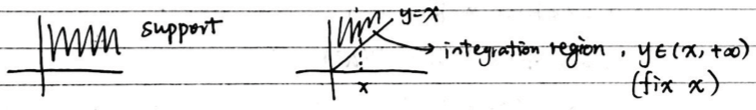
\includegraphics{0-1}
	\end{center}
	\item \textbf{Independence: } If $X,Y$ are independent, then 
	\begin{gather*}
		\textbf{Continuous: }\quad \quad f(x,y) = f_X(x)f_Y(y)\\
		\textbf{Discrete: }\quad \quad P(X=x, Y=y) = P(X=x) P(Y=y)
	\end{gather*}
	\item \textbf{Convolution: } assume $X,Y$ are independent
	\begin{gather*}
		\textbf{Discrete: }\quad \quad P_{X+Y}(a) = \sum\limits_y P_X(a-y)P_Y(y) = \sum\limits_x P_X(x)P_Y(a-x)\\
		\textbf{Continuous: }\quad \quad f_{X+Y}(a) = \int_y f_X(a-y)f_Y(y)dy = \int_y f_X(x)f_Y(a-x)dx\\
		\textbf{MGF: }\text{we can use this} \quad \quad M_{X+Y}(t) = M_X(t) M_Y(t) \longrightarrow \text{then identify dist of X+Y from mgf} 
	\end{gather*}
\end{itemize}
\subsection*{Conditional distribution}
\begin{align*}
	\textbf{Discrete} \quad \quad
	& P_{X|Y=y}(x|y) = \frac{P_{X,Y}(x,y)}{P_Y(y)} = \frac{P(X=x, Y=y)}{P(Y=y)}\\
  & \Rightarrow \sum\limits_y P_{X,Y}(x,y) = \sum\limits_y P_{X|Y=y}(x|y) \cdot P_Y(y)\\
  \textbf{Continuous} \quad \quad & f_{X|Y=y}(x|y) = \frac{f_{X,Y}(x,y)}{f_Y(y)}\\
  & \Rightarrow f_X(x) = \int_y f(x,y)dy = \int_y f_{X|Y=y}(x|y)\cdot f_Y(y)dy
\end{align*}
\subsubsection*{Conditional Expectation}
\begin{align*}
	& E[X|Y=y] = \int_x xf(x|y) dx\\
	& E[X|Y]: \text{compute } E[X|Y=y] \text{ first, replace $y$ with $Y$}
\end{align*}
\subsection*{Ordered Statistics}
Consider $X_1, X_2, \cdots, X_n \quad \quad X_{(j)}$ = j-th smallest
\begin{align*}
	F_{\max(X_i)}(t) & = P(\max X_i \leq t) = P(X_1 \leq t)\cdot P(X_2 \leq t) \cdots P(X_n \leq t)\\
	& = [F_X(t)]^n \quad \quad \quad
	\boxed{f_{\max X_i}(t) = nF(t)^{n-1} f_X(t)}\\
	 F_{\min(X_i)}(t) & = 1 - P(\min x_i \geq t) = 1-P(X_1 \geq t)\cdot P(X_2 \geq t) \cdots P(X_n \geq t)\\
	 & = 1 - [1 - F_X(t)]^n \quad \quad \quad \boxed{f_{\min X_i}(t) = n[1 - F(t)]^{n-1} f_X(t)}
\end{align*}
\textbf{General:} $j$-th order statistic
\begin{equation*}
	f_{x(j)}(t) = \binom{n}{j-1,1,n-j} F_X(t)^{j-1}\cdot f_X(t) \cdot [1-F_X(t)]^{n-j}
\end{equation*}
\subsection*{Expectation and Variance}
\begin{gather*}
	\textbf{Law of Total Expectation: } E[X] = E[E[X|Y]]\\
\textbf{Law of Total Variance: } Var(X) = E[Var(X|Y)] + Var[E(X|Y)]
\end{gather*}
\subsubsection*{Expectation}
\begin{enumerate}[label=\protect\circled{\arabic*}]
	\item linearity of expectation
	\item How to compute
	\begin{enumerate}
		\item LOTUS or definition (use density to integrate)
		\item MGF: $M^{(n)}(0) = E[X^n]$ or by recognition
		\item $E[X^2] = Var[X] + E[X]^2$
		\item Tail probability X is non-neg R.V. $(x>0)$ then $E[X] = \sum\limits_{t=0}^\infty P(X \geq t)$ \textit{or} $= \int\limits_0^\infty P(X \geq t) dt$
	\end{enumerate}
\end{enumerate}
\subsubsection*{Variance}
\begin{enumerate}[label=\protect\circled{\arabic*}]
	\item $Var(X_1 + X_2 + \cdots + X_n) = \sum\limits_{i=1}^n Var(X_i) + \sum\limits_{i \neq j} Cov(X_i, X_j)$
	\begin{center}
		if $X_i, X_j$ identical (not independent) $ = n Var(X_i) + n(n-1)Cov(X_i, X_j) \quad \quad i\neq j$
	\end{center}
	\item \textbf{Covariance: }
	\begin{align*}
		Cov(X,Y) & = E[XY] - E[X]E[Y]\\
		Cov(X,c) & = 0 \quad \quad c \textit{ is a constant}\\
		Cov(X+Y,Z) & = Cov(X,Z) + Cov(Y,Z)\\
		Cov(cX,dZ) & = cd \cdot Cov(X,Z) 
	\end{align*}
	\item \textbf{Correlation Coefficient:}
	\begin{equation*}
		\rho(X,Y) = \frac{Cov(X,Y)}{\sqrt{Var(X) Var(Y)}} = \frac{Cov(X,Y)}{\sigma_x \sigma_y}
	\end{equation*}
\end{enumerate}
\subsection*{Limit Theorems}
\subsubsection*{Markov's Inequality}
For any non-negative random variable $X$
\begin{equation*}
	P(X \geq a) \leq \frac{E(X)}{a} \tag{for \underline{any} $a > 0$}
\end{equation*}
\begin{proof}
	Let $X \geq 0$ a random variable and let $a > 0$.
	Define new random variable from $X$ as $Y_a$
	\begin{gather*}
		Y_a =
		\begin{cases}
 		0 & \text{if }	X < a\\
 		a & \text{if }	X \geq a\\
		 \end{cases}\\
		0 \leq Y_a \leq X \Longrightarrow \underbrace{E[Y_a]}_{a\cdot P(X \geq a)} \leq E[X]\\
		E[Y_a] = 0 \cdot P(Y_a < a) + a\cdot P(X \geq a)\\
		 E[Y_a] = a\cdot P(X \geq a) \leq E[X] \Longrightarrow \boxed{P(X \geq a) \leq \frac{E(X)}{a}}
	\end{gather*}
\end{proof}
\subsubsection*{Chebyshev's Inequality}
For any random variable Y with mean $\mu_y$ and variance $\sigma_y^2$
\begin{equation*}
	P(|Y - \mu)y| \geq c) \leq \frac{\sigma_y^2}{c^2} \tag{for \underline{any} $c > 0$}
\end{equation*}
\begin{proof}
	\begin{gather*}
		P(|Y - \mu_y)| \geq c) = P(\underbrace{|Y - \mu_y)|^2}_{=X} \geq c^2)\\
		P(|Y - \mu_y)|^2 \geq c^2) \leq \frac{E[|Y - \mu_y|^2]}{c^2} = \frac{\sigma_y^2}{c^2}
	\end{gather*}
\end{proof}
This is the same as
\begin{itemize}[label={--}]
	\item $P(|Y - \mu_y| \geq k \sigma_y) \leq \frac{1}{k^2}$
	\item $P(|Y - \mu_y| \leq k \sigma_y) \geq \underbrace{1- \frac{1}{k^2}}_{\text{very conservative}}$
\end{itemize}
\subsubsection*{Weak Law of Large Numbers}
If $X_1, X_2, \cdots$ are $i.i.d.$ with a mean $\mu$
\begin{equation*}
	\text{then} \qquad \mathlarger{\mathlarger{\Lim{n \rightarrow \infty}}} {\large P}\bigg( \bigg| \frac{X_1 + X_2 + \cdots + X_n}{n} - \mu \bigg| \geq \epsilon \bigg) = 0
\end{equation*}





	
\end{document}
